% Options for packages loaded elsewhere
\PassOptionsToPackage{unicode}{hyperref}
\PassOptionsToPackage{hyphens}{url}
%
\documentclass[
]{book}
\usepackage{amsmath,amssymb}
\usepackage{lmodern}
\usepackage{iftex}
\ifPDFTeX
  \usepackage[T1]{fontenc}
  \usepackage[utf8]{inputenc}
  \usepackage{textcomp} % provide euro and other symbols
\else % if luatex or xetex
  \usepackage{unicode-math}
  \defaultfontfeatures{Scale=MatchLowercase}
  \defaultfontfeatures[\rmfamily]{Ligatures=TeX,Scale=1}
\fi
% Use upquote if available, for straight quotes in verbatim environments
\IfFileExists{upquote.sty}{\usepackage{upquote}}{}
\IfFileExists{microtype.sty}{% use microtype if available
  \usepackage[]{microtype}
  \UseMicrotypeSet[protrusion]{basicmath} % disable protrusion for tt fonts
}{}
\makeatletter
\@ifundefined{KOMAClassName}{% if non-KOMA class
  \IfFileExists{parskip.sty}{%
    \usepackage{parskip}
  }{% else
    \setlength{\parindent}{0pt}
    \setlength{\parskip}{6pt plus 2pt minus 1pt}}
}{% if KOMA class
  \KOMAoptions{parskip=half}}
\makeatother
\usepackage{xcolor}
\usepackage{longtable,booktabs,array}
\usepackage{calc} % for calculating minipage widths
% Correct order of tables after \paragraph or \subparagraph
\usepackage{etoolbox}
\makeatletter
\patchcmd\longtable{\par}{\if@noskipsec\mbox{}\fi\par}{}{}
\makeatother
% Allow footnotes in longtable head/foot
\IfFileExists{footnotehyper.sty}{\usepackage{footnotehyper}}{\usepackage{footnote}}
\makesavenoteenv{longtable}
\usepackage{graphicx}
\makeatletter
\def\maxwidth{\ifdim\Gin@nat@width>\linewidth\linewidth\else\Gin@nat@width\fi}
\def\maxheight{\ifdim\Gin@nat@height>\textheight\textheight\else\Gin@nat@height\fi}
\makeatother
% Scale images if necessary, so that they will not overflow the page
% margins by default, and it is still possible to overwrite the defaults
% using explicit options in \includegraphics[width, height, ...]{}
\setkeys{Gin}{width=\maxwidth,height=\maxheight,keepaspectratio}
% Set default figure placement to htbp
\makeatletter
\def\fps@figure{htbp}
\makeatother
\setlength{\emergencystretch}{3em} % prevent overfull lines
\providecommand{\tightlist}{%
  \setlength{\itemsep}{0pt}\setlength{\parskip}{0pt}}
\setcounter{secnumdepth}{5}
\usepackage{booktabs}
\usepackage{amsthm}
\makeatletter
\def\thm@space@setup{%
  \thm@preskip=8pt plus 2pt minus 4pt
  \thm@postskip=\thm@preskip
}
\makeatother
\ifLuaTeX
  \usepackage{selnolig}  % disable illegal ligatures
\fi
\usepackage[]{natbib}
\bibliographystyle{plainnat}
\IfFileExists{bookmark.sty}{\usepackage{bookmark}}{\usepackage{hyperref}}
\IfFileExists{xurl.sty}{\usepackage{xurl}}{} % add URL line breaks if available
\urlstyle{same} % disable monospaced font for URLs
\hypersetup{
  pdftitle={GEOG0030: Geocomputation},
  pdfauthor={Justin van Dijk},
  hidelinks,
  pdfcreator={LaTeX via pandoc}}

\title{GEOG0030: Geocomputation}
\author{Justin van Dijk}
\date{Last modified: 2022-11-25}

\begin{document}
\maketitle

{
\setcounter{tocdepth}{1}
\tableofcontents
}
\hypertarget{module-overview}{%
\chapter*{Module Overview}\label{module-overview}}
\addcontentsline{toc}{chapter}{Module Overview}

\hypertarget{module-introduction}{%
\chapter*{Module Introduction}\label{module-introduction}}
\addcontentsline{toc}{chapter}{Module Introduction}

\begin{center}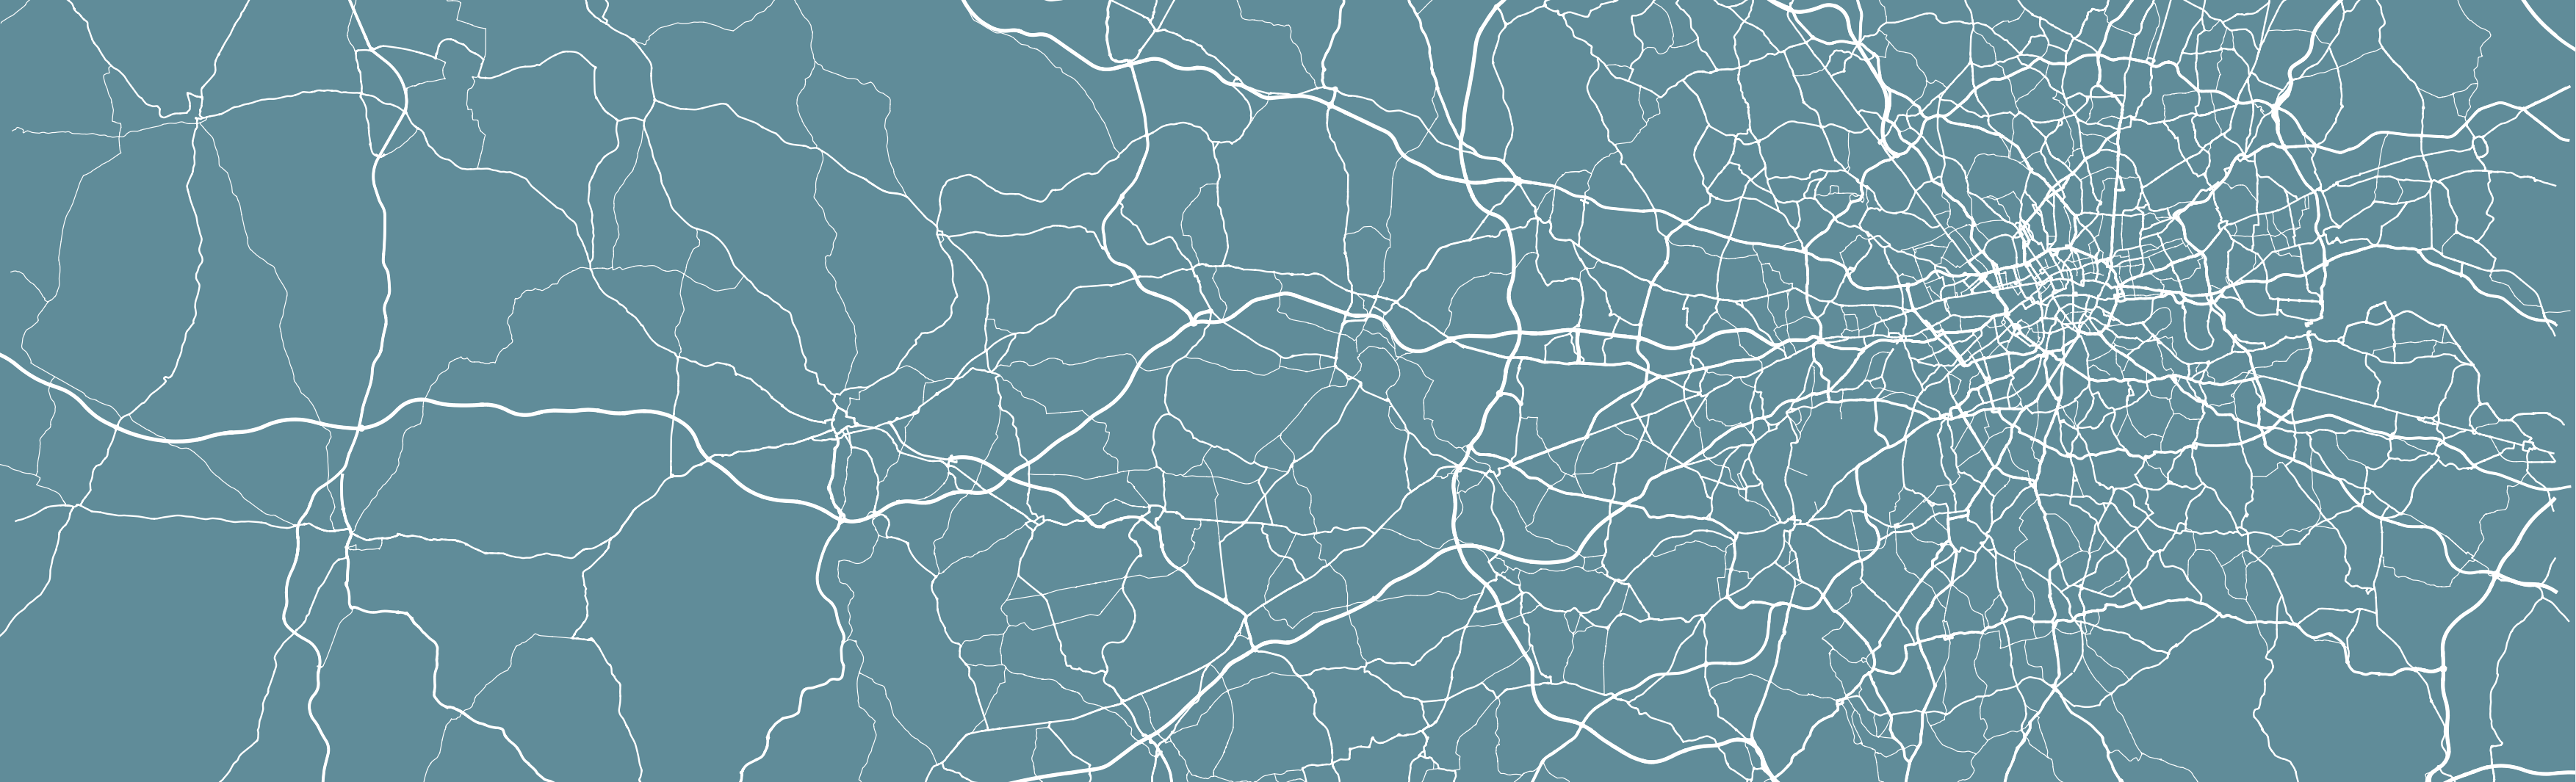
\includegraphics[width=1\linewidth]{images/general/geocomputation_welcome} \end{center}

\hypertarget{welcome}{%
\section*{Welcome}\label{welcome}}
\addcontentsline{toc}{section}{Welcome}

Welcome to \textbf{Geocomputation}. This module will introduce you both to the principles of spatial analysis as well as provide you with a comprehensive introduction to the use of programming. Over the next ten weeks, you will learn about the theory, methods and tools of spatial analysis through relevant case studies. We will start by using QGIS before moving to the R programming language. You will learn how to find, manage and clean spatial, demographic and socioeconomic datasets, and then analyse them using core spatial and statistical analysis techniques.

\hypertarget{moodle}{%
\section*{Moodle}\label{moodle}}
\addcontentsline{toc}{section}{Moodle}

\href{https://moodle.ucl.ac.uk/}{Moodle} is the central point of contact for GEOG0030 and it is where all important information will be communicated such as key module and assessment information. This workbook contains links to all reading material as well as the content of all computer tutorials

\hypertarget{module-overview-1}{%
\section*{Module overview}\label{module-overview-1}}
\addcontentsline{toc}{section}{Module overview}

The topics covered over the next ten weeks are:

\begin{longtable}[]{@{}
  >{\raggedright\arraybackslash}p{(\columnwidth - 4\tabcolsep) * \real{0.1212}}
  >{\raggedright\arraybackslash}p{(\columnwidth - 4\tabcolsep) * \real{0.3030}}
  >{\raggedright\arraybackslash}p{(\columnwidth - 4\tabcolsep) * \real{0.5758}}@{}}
\toprule()
\begin{minipage}[b]{\linewidth}\raggedright
Week
\end{minipage} & \begin{minipage}[b]{\linewidth}\raggedright
Section
\end{minipage} & \begin{minipage}[b]{\linewidth}\raggedright
Topic
\end{minipage} \\
\midrule()
\endhead
1 & Foundational Concepts & \href{geocomputation-an-introduction.html}{Geocomputation: An Introduction} \\
2 & Foundational Concepts & \href{giscience-and-gis-software.html}{GIScience and GIS software} \\
3 & Foundational Concepts & \href{cartography-and-visualisation.html}{Cartography and Visualisation} \\
4 & Foundational Concepts & \href{programming-for-data-analysis.html}{Programming for Data Analysis} \\
5 & Foundational Concepts & \href{programming-for-spatial-analysis.html}{Programming for Spatial Analysis} \\
& \textbf{Reading week} & \textbf{Reading week} \\
6 & Core Spatial Analysis & \href{analysing-spatial-patterns-i-geometric-operations-and-spatial-queries.html}{Analysing Spatial Patterns I: Geometric Operations and Spatial Queries} \\
7 & Core Spatial Analysis & \href{analysing-spatial-patterns-ii-spatial-autocorrelation.html}{Analysing Spatial Patterns II: Spatial Autocorrelation} \\
8 & Core Spatial Analysis & \href{analysing-spatial-patterns-iii-point-pattern-analysis.html}{Analysing Spatial Patterns III: Point Pattern Analysis} \\
9 & Advanced Spatial Analysis & \href{rasters-zonal-statistics-and-interpolation.html}{Rasters, Zonal Statistics and Interpolation} \\
10 & Advanced Spatial Analysis & \href{transport-network-analysis.html}{Transport Network Analysis} \\
\bottomrule()
\end{longtable}

\hypertarget{troubleshooting}{%
\section*{Troubleshooting}\label{troubleshooting}}
\addcontentsline{toc}{section}{Troubleshooting}

Spatial analysis can yield fascinating insights into geographical relationships, albeit at times it can be challenging, particularly when we combine this with learning how to program at the same time. You will most likely encounter many error messages, experience software crashes, and spend hours to identify bugs in your code. However, the rewards of learning how to programmatically solve complex spatial problems will be very much worth it in the end.

If you need specific assistance with this course please:

\begin{itemize}
\tightlist
\item
  Ask a question at the end of a lecture or during the computer practical.
\item
  Attend the Department's \textbf{Coding Therapy sessions} that are run on a weekly basis.
\item
  Check the \href{https://moodle.ucl.ac.uk/}{Moodle} assessment tab for queries relating to this module's assessment.
\end{itemize}

If after pursuing all these avenues you still need help, you can book into our office hours. You can use an office hour to discuss a geographical concept in relation to the material, assessment or for any personal matters relevant to the completion of the module.

\hypertarget{acknowledgements}{%
\section*{Acknowledgements}\label{acknowledgements}}
\addcontentsline{toc}{section}{Acknowledgements}

This year's workbook is updated and compiled using:

\begin{itemize}
\tightlist
\item
  The \href{https://jo-wilkin.github.io/GEOG0030/coursebook/index.html}{GEOG0030: Geocomputation 2021-2021} workbook as created and compiled by Dr Jo Wilkin.
\item
  The \href{https://jtvandijk.github.io/GEOG0030_20212022/}{GEOG0030: Geocomputation 2021-2022} workbook.
\end{itemize}

The datasets used in this workbook contain:

\begin{itemize}
\tightlist
\item
  National Statistics data © Crown copyright and database right {[}2015{]} (Open Government Licence)
\item
  Ordnance Survey data © Crown copyright and database right {[}2015{]}
\item
  Public Health England © Crown copyright 2021
\item
  Crime data obtained from \href{https://data.police.uk/}{data.police.uk} (Open Government Licence)
\end{itemize}

\hypertarget{additional-resources}{%
\chapter*{Additional Resources}\label{additional-resources}}
\addcontentsline{toc}{chapter}{Additional Resources}

\hypertarget{data-sources}{%
\chapter{Data Sources}\label{data-sources}}

Below you will find a list of resources that you might want to explore when sourcing data for your coursework assignment or your dissertation. This is by no means an exhaustive list, but simply contains some suggestions of websites that you may want to use.

\textbf{Note}
You are \textbf{not limited} to using these datasets for your coursework assignment or your dissertation.

\hypertarget{open-data}{%
\section{Open Data}\label{open-data}}

The following websites contain Open Data or link to Open Data from several respectable data providers:

\begin{itemize}
\tightlist
\item
  \href{http://insideairbnb.com/get-the-data.html}{AirBnB Data}
\item
  \href{https://docs.ropensci.org/bikedata/}{Bike Docking Data (ready for R)}
\item
  \href{https://camdenairaction.wordpress.com/2017/02/20/schools-monitoring-project-spring-2017/}{Camden Air Action}
\item
  \href{https://data.cdrc.ac.uk/}{Consumer Data Research Centre}
\item
  \href{https://environment.data.gov.uk/}{DEFRA}
\item
  \href{https://www.diva-gis.org/}{DIVA-GIS}
\item
  \href{https://digimap.edina.ac.uk/}{Edina (e.g.~OS mastermap)}
\item
  \href{https://ec.europa.eu/eurostat/statistics-explained/index.php/Tourism_statistics}{EU Tourism Data}
\item
  \href{https://ec.europa.eu/eurostat}{Eurostat}
\item
  \href{https://www.geofabrik.de/}{Geofabrik (OSM data)}
\item
  \href{https://rp5.ru/Weather_in_the_world}{Global Weather Data}
\item
  \href{https://datasetsearch.research.google.com/}{Google Dataset Search}
\item
  \href{https://github.com/RamiKrispin/coronavirus}{Johns Hopkins COVID19 Data (ready for R}
\item
  \href{https://www.londonair.org.uk/LondonAir/Default.aspx}{King's College Data on Air Pollution}
\item
  \href{https://data.london.gov.uk/}{London Data Store}
\item
  \href{https://www.ft.com/content/6f381ad4-fef7-11e9-be59-e49b2a136b8d}{London Tube PM2.5 Levels}
\item
  \href{https://earthdata.nasa.gov/}{NASA EARTHDATA}
\item
  \href{https://sedac.ciesin.columbia.edu/}{NASA SocioEconomic Data and Applications Center (SEDAC)}
\item
  \href{https://nhs-r-community.github.io/NHSRdatasets/}{NHS Data (ready for R)}
\item
  \href{https://www.nomisweb.co.uk/}{nomis Official Census and Labour Market Statistics}
\item
  \href{https://geoportal.statistics.gov.uk/}{Office for National Statistics Geoportal}
\item
  \href{https://www.ons.gov.uk/}{Office for National Statistics}
\item
  \href{https://opentopography.org/}{Open Topography}
\item
  \href{https://www.nature.com/articles/s41597-020-0397-7}{Tesco Store Data (London)}
\item
  \href{https://cycling.data.tfl.gov.uk/}{TfL Cycling Data}
\item
  \href{https://tfl.gov.uk/info-for/open-data-users/our-open-data?intcmp=3671\#on-this-page-2}{TfL Open Data}
\item
  \href{https://github.com/rfordatascience/tidytuesday}{Tidy Tuesday Data (not exclusively spatial data)}
\item
  \href{https://movement.uber.com/?lang=en-GB}{Uber Travel Time Data}
\item
  \href{https://coronavirus.data.gov.uk/}{UK COVID19 Data}
\item
  \href{https://ukdataservice.ac.uk/}{UK Data Service}
\item
  \href{https://www.census.gov/data.html}{US Census Data}
\item
  \href{http://us-cities.survey.okfn.org/}{US City Open Data Census}
\item
  \href{https://earthexplorer.usgs.gov/}{USGS Earth Explorer}
\item
  \href{https://github.com/wpgp}{WorldPop GitHub}
\item
  \href{https://www.worldpop.org/}{WorldPop}
\end{itemize}

Some other websites that could be helpful:

\begin{itemize}
\tightlist
\item
  \href{https://github.com/awesomedata/awesome-public-datasets}{Awesome Public Datasets}; general collection of datasets, although not limited to spatial data.
\item
  \href{https://freegisdata.rtwilson.com/}{Free GIS data}; long list with lots of GIS datasets on many different topics and covering many different areas.
\end{itemize}

\hypertarget{safeguarded-data}{%
\section{Safeguarded Data}\label{safeguarded-data}}

Undergraduate students can also apply for a \textbf{Safeguarded} dataset held by the \href{https://www.cdrc.ac.uk/}{Consumer Data Research Centre}. There is a process to access these \textbf{Safeguarded} datasets, which is detailed on the \href{https://data.cdrc.ac.uk/using-our-data-services}{CDRC website}. Please be aware that it normally takes 4-5 weeks for your application to be processed.

As part of the process, you will need to say in your application why you want that specific dataset and what you are planning to do with it. You will also need to have at least thought about the ethical implications of using that data and provide this with your data application (alongside your standard ethics application).

Some of the datasets held by the CDRC that you can apply for are:

\begin{itemize}
\tightlist
\item
  \href{https://data.cdrc.ac.uk/dataset/bicycle-sharing-system-docking-station-observations}{Bicycle Sharing System Docking Station Observations}
\item
  \href{https://data.cdrc.ac.uk/dataset/cdrc-modelled-ethnicity-proportions-lsoa-geography}{CDRC Modelled Ethnicity Proportions - LSOA Geography}
\item
  \href{https://data.cdrc.ac.uk/dataset/fca-financial-lives-survey}{FCA Financial Lives Survey}
\item
  \href{https://data.cdrc.ac.uk/dataset/local-data-company-smartstreetsensor-footfall-data-\%E2\%80\%93-research-aggregated-data}{Local Data Company - SmartStreetSensor Footfall Data -- Research Aggregated data}
\item
  \href{https://data.cdrc.ac.uk/dataset/nhs-hospital-admission-rates-ethnic-group-and-other-characteristics}{NHS Hospital Admission Rates by Ethnic Group and other Characteristics}
\item
  \href{https://data.cdrc.ac.uk/dataset/speedchecker-broadband-internet-speed-tests}{Speedchecker Broadband Internet Speed Tests}
\end{itemize}

\textbf{Note}
Given that the application can take several weeks, the Safeguarded CDRC datasets may be useful for your dissertation work but probably not for the GEOG0030 coursework assignment. However, any of the CDRC datasets that are marked as \textbf{Open Data} do not require this application process and you can download these datasets directly after registering on the website.

\end{document}
